\subsection{Data}


We construct a collection of relatively high-quality video clips with text descriptions with video filters and recaption models. % based on CogVLM2~\cite{wang2023cogvlm}. 
After filtering, approximately 35M single-shot clips remain, with each clip averaging about 6 seconds. We additionally use 2B images filtered with aesthetics score from LAION-5B~\citep{schuhmann2022laion} and COYO-700M~\citep{kakaobrain2022coyo-700m} datasets to assist training.



\paragraph{Video Filtering.}

Video generation models should capture the dynamic nature of the world. However, raw video data often contains significant noise for two intrinsic reasons: First, the artificial editing during video creation can distort the true dynamic information; Second, video quality may suffer due to filming issues such as camera shakes or using subpar equipment. In addition to the intrinsic quality of the videos, we also consider how well the video data supports model training. 
Videos with minimal dynamic information or lacking connectivity in dynamic aspects are considered detrimental. 
Consequently, we have developed a set of negative labels, which include:

\begin{itemize}
    \item \textbf{Editing}: Videos that have undergone noticeable artificial processing, such as re-editing and special effects, which compromise the visual integrity.
    \item \textbf{Lack of Motion Connectivity}: Video segments with transitions that lack coherent motion, often found in artificially spliced videos or those edited from static images.
    \item \textbf{Low Quality}: Poorly shot videos with unclear visuals or excessive camera shake.
    \item \textbf{Lecture Type}: Videos focusing primarily on a person continuously talking with minimal effective motion, such as educational content, lectures, and live-streamed discussions.
    \item \textbf{Text Dominated}: Videos containing a large amount of visible text or primarily focusing on textual content.
    \item \textbf{Noisy Screenshots}: Videos captured directly from phone or computer screens, often characterized by poor quality.
\end{itemize}

We first sample 20,000 videos and label each video as positive or negative by their quality.
Using these annotations, we train 6 filters based on Video-LLaMA~\citep{zhang2023video} to screen out low-quality video data. Examples of negative labels and the classifier's performance on the test set can be found in \cref{ap:data_filtering_details}.
In addition, we calculate the optical flow scores and image aesthetic scores of all training videos, and dynamically adjust their threshold during training to ensure the dynamic and aesthetic quality of generated videos. 




\paragraph{Video Captioning.}
Video-text pairs are essential for the training of text-to-video generation models.
However, most video data does not come with corresponding descriptive text. Therefore, it is necessary to label the video data with comprehensive textual descriptions. 
Currently, there are some video caption datasets available, such as Panda70M~\citep{chen2024panda}, COCO Caption~\citep{lin2014microsoft}, and WebVid~\cite{bain2021frozen}. 
However, the captions in these datasets are usually very short and fail to describe the video's content comprehensively. 




\begin{figure}[tb]
  \centering
  % 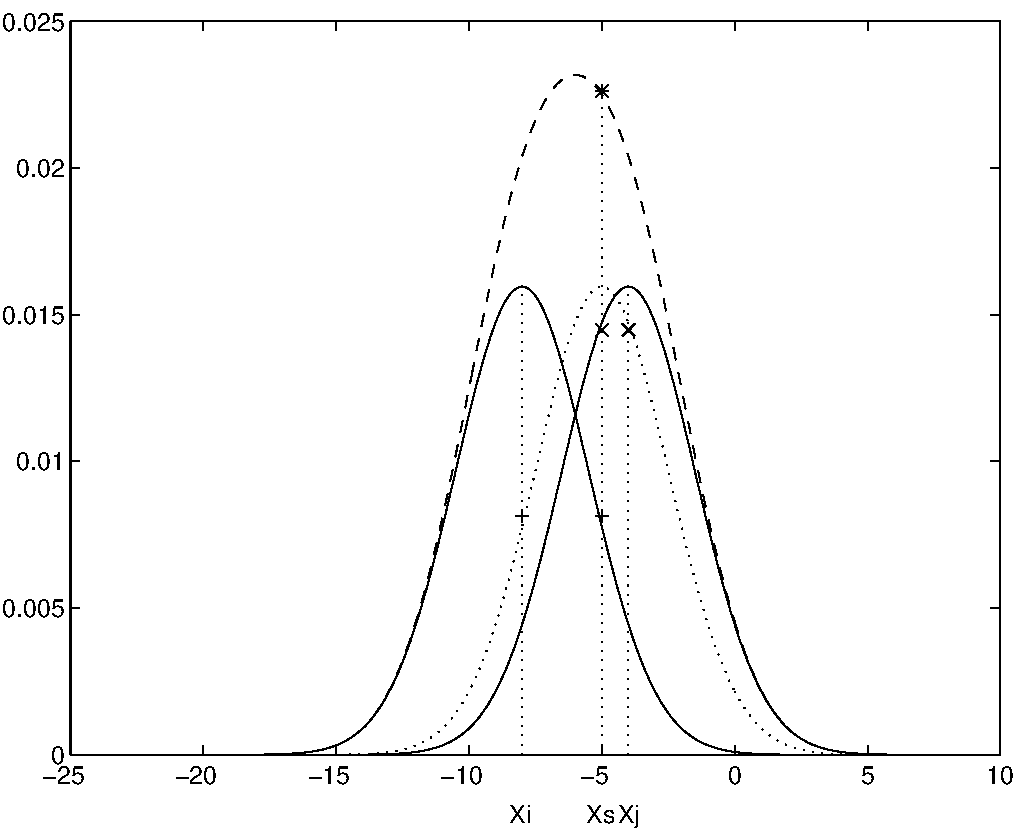
\includegraphics[height=6.5cm]{eijkel2}
  % \fbox{\rule{0pt}{0.8in} \rule{.95\linewidth}{0pt}}
  %\includesvg[inkscapelatex=false, width = 1\linewidth]{images/pipeline_frosting_largefont}
  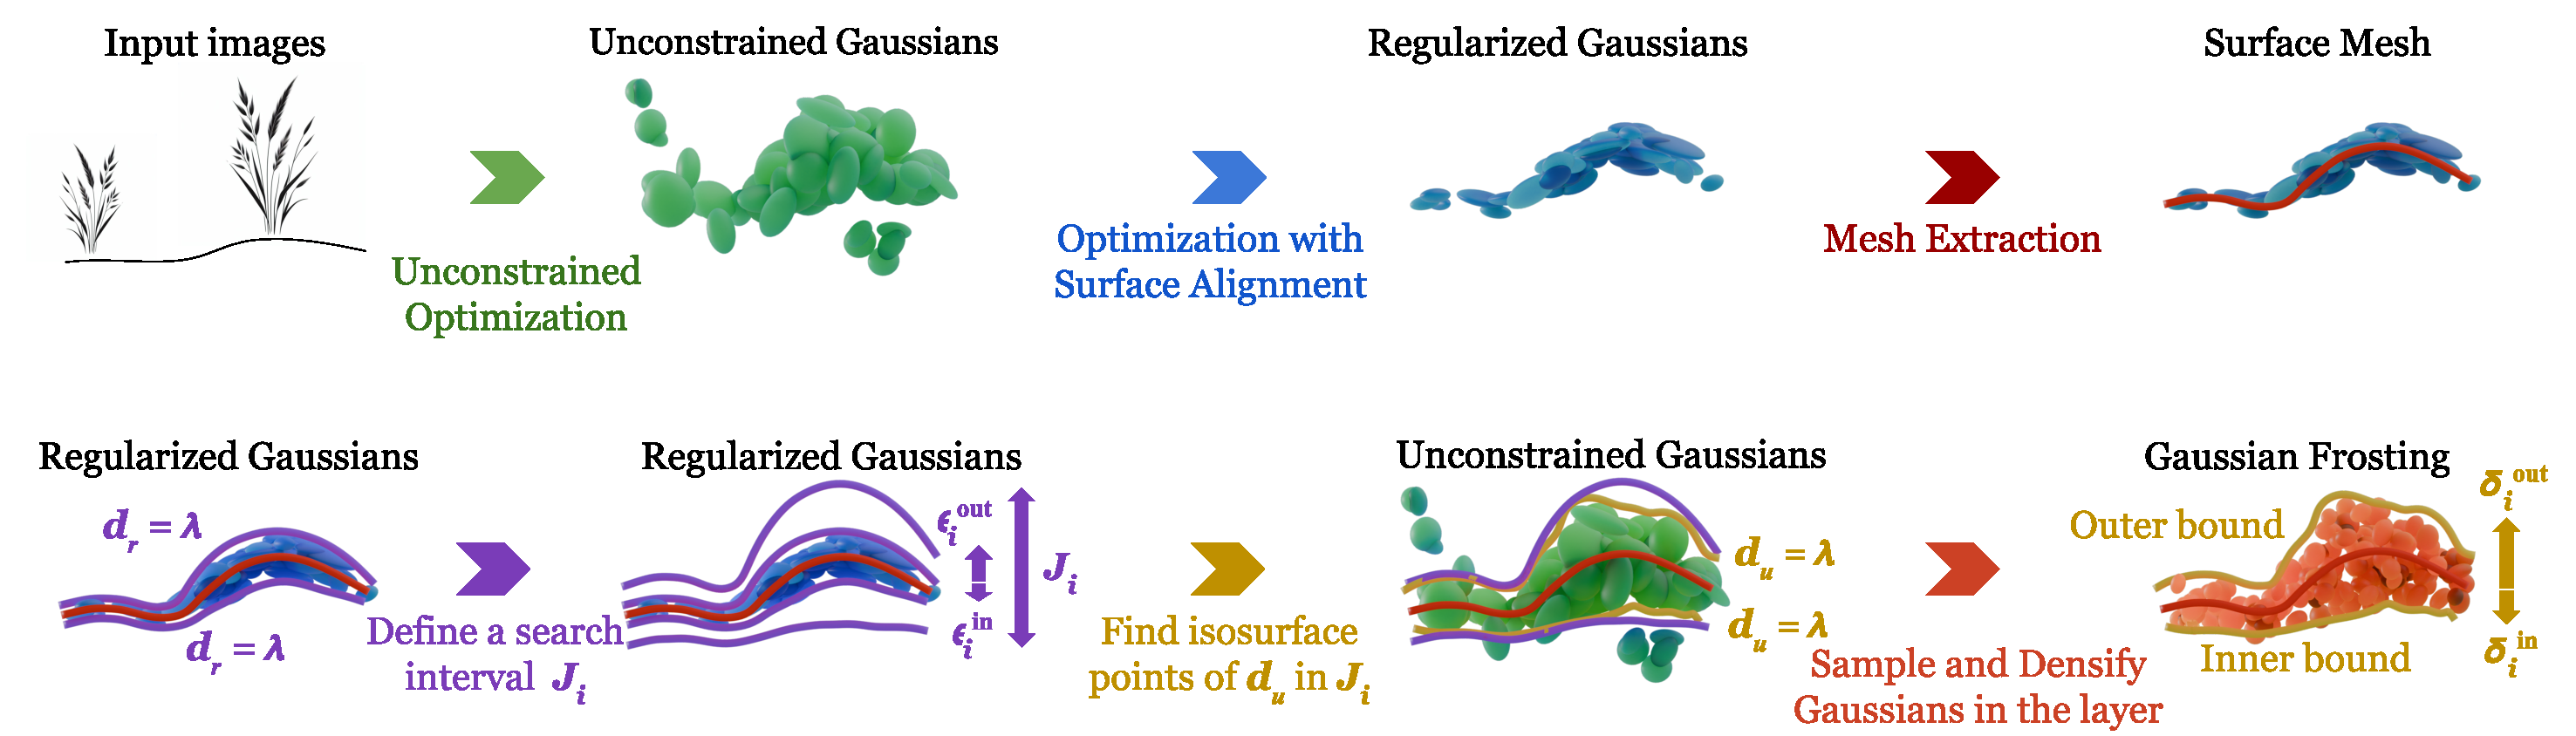
\includegraphics[width=\linewidth]{images/pipeline_frosting_largefont.pdf}
  \caption{
  \textbf{Creating a Layer of Gaussian Frosting.} To build our proposed Frosting representation, we start by optimizing a Gaussian Splatting representation using a rendering loss without any additional constraint, to let Gaussians position themselves. We refer to these Gaussians as \emph{unconstrained}. We then regularize these Gaussians to enforce their alignement with the surface, and extract a mesh that will serve as a basis for the Frosting. Next, we use the misalignment of surface-aligned Gaussians to identify areas where more volumetric rendering is needed, and we build search intervals $J_i$ around the mesh's vertices $\vec{v_i}$. Finally, we use the density function of the unconstrained Gaussians to refine the intervals, resulting in a Frosting layer. We finally sample a novel, densified set of Gaussians inside the layer.
}
  \label{fig:frosting-pipeline}
\end{figure}

%\paragraph{.} 
To generate high-quality video caption data, we establish a \textit{Dense Video Caption Data Generation} 
%complex data generation 
pipeline, as detailed in Figure~\ref{fig:video_caption_gen}.  
The main idea is to generate video captions with the help of image captions. %

First, we use the video caption model from~\citet{chen2024panda} to generate short captions for the videos. 
Then, we employ the image recaptioning model CogVLM~\citep{wang2023cogvlm} used in CogView3~\citep{zheng2024cogview3} to create dense image captions for each frame.  
Subsequently, we use GPT-4 to summarize all the image captions to produce the final video caption. 
To accelerate the generation from image captions to video captions, we fine-tune a LLaMA2~\citep{touvron2023llama} using the summary data generated by GPT-4~\citep{GPT4}, enabling large-scale video caption data generation. Additional details regarding the video caption data generation process can be found in Appendix~\ref{ap:video_caption_gen}.


%We thus propose to build a pipeline to generate video captions from image captions and then fine-tune an end-to-end video captioning model to obtain more dense video captions. 
%Our final video captioning model can generate more detailed descriptions of videos, further enhancing the quality of video generation \citep{betker2023improving}.
 
%The pipeline above generates the caption data that is used to trained the \model model introduced in this report. 
To further accelerate video recaptioning, we also fine-tune an end-to-end video understanding model CogVLM2-Caption\footnote{The CogVLM2-Caption model weight is openly available at 
\href{https://huggingface.co/THUDM/cogvlm2-llama3-caption}{https://huggingface.co/THUDM/cogvlm2-llama3-caption}.
%\url{https://huggingface.co/THUDM/cogvlm2-llama3-caption}.
}, based on the CogVLM2-Video~\citep{hong2024cogvlm2} and Llama3~\citep{llama3modelcard}, by using the dense caption data generated from the aforementioned pipeline. 
% The video caption data generated by CogVLM2-Caption is used to train the next generation of \model. 
%This dense video captions. % as described above through the pipeline method. 
Examples of video captions generated by this end-to-end CogVLM2-Caption model are shown in \cref{fig:v2t} and Appendix~\ref{ap:video_caption_example}. CogVLM2-Caption can provide detailed descriptions of video content and object changes. Interestingly, we find that we can perform video-to-video generation by connecting CogVideoX and CogVLM2-Caption, as detailed in ~\cref{ap:v2v}.

% In Appendix~\ref{ap:v2v}, we also present some examples of video generation where a video is first input into CogVLM2-Caption to generate captions, which are then used as input for \model to generate new videos, effectively achieving video-to-video generation.



% In Appendix~\ref{ap:v2v}, we show video-to-video generation by using CogVLM2-Caption for video caption, then \model to generate new videos. The cogvlm2-caption can capture almost all the details in the video, so \model can rely solely on the caption to effectively reconstruct the original video.



